\documentclass[a4paper,12pt]{article}
\usepackage[left=2.5cm,right=2.5cm,top=0cm]{geometry}
\usepackage{tikz}

\usetikzlibrary{shapes.geometric}
\usepackage{hyperref}
\hypersetup{
    colorlinks=false,
    urlbordercolor=white
    }
\usepackage[none]{hyphenat}
\title{Monthly Maths Circle India Challenge}
% \author{Disha Kuzhively}
% \email{disha.jk@icts.res.in}
\date{Solutions\\March 2024}
\begin{document}
\maketitle
\thispagestyle{empty}
\begin{enumerate}
    \item[Solution 1.] Following are two of the many ways in which the L-shape can be tiled using congruent shapes, dividing the L-shape into eight equal parts.
    \begin{figure}[h]
        \centering
        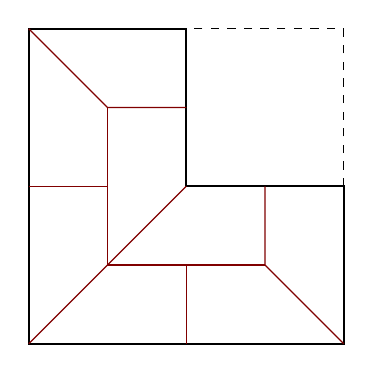
\begin{tikzpicture}
    \draw[black,thick] (0,0) -- (4,0) -- (4,2) --  (2,2) -- (2,4) -- (0,4) -- cycle;
    \draw[dashed] (4,2) -- (4,4) -- (2,4);
    \draw[red!50!black] (0,0) -- (2,2);
    \draw[red!50!black] (0,4) -- (1,3) -- (2,3);
    \draw[red!50!black] (4,0) -- (3,1) -- (3,2);
    \draw[red!50!black] (1,3) -- (1,1) -- (3,1);
    \draw[red!50!black] (2,0) -- (2,1);
    \draw[red!50!black] (0,2) -- (1,2);
\end{tikzpicture}
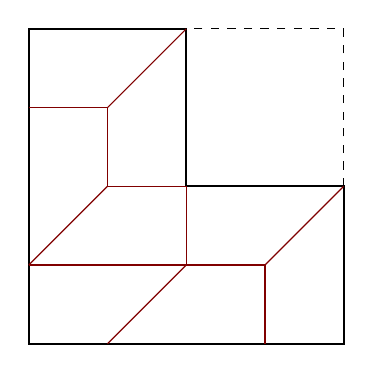
\begin{tikzpicture}
    \draw[black,thick] (0,0) -- (4,0) -- (4,2) --  (2,2) -- (2,4) -- (0,4) -- cycle;
    \draw[dashed] (4,2) -- (4,4) -- (2,4);
    \draw[red!50!black] (0,3) -- (1,3) -- (1,2) -- (2,2) -- (2,1) -- (3,1) -- (3,0);
    \draw[red!50!black] (1,2) -- (0,1);
    \draw[red!50!black] (1,3) -- (2,4);
    \draw[red!50!black] (2,1) -- (1,0);
    \draw[red!50!black] (3,1) -- (4,2);
    \draw[red!50!black] (0,1) -- (2,1);
\end{tikzpicture}

\begin{tikzpicture}
    \filldraw[red!50!black] (0,0) -- (2,0) -- (2,1) -- (1,1) -- cycle;
\end{tikzpicture}                
    \end{figure}

\end{enumerate}
\end{document}